\documentclass{article}
\usepackage{enumerate, tikz, fancyhdr, framed, color}
\usepackage[margin=1.25in]{geometry}

% =============================================================

\pagestyle{fancy}
\definecolor{shadecolor}{gray}{0.95}
\lhead{Lucas Freitas and Angela Li}
\chead{} 
\rhead{\thepage} 
\lfoot{\small Computer Science 181} 
\cfoot{} 
\rfoot{\footnotesize Probabilistic Graphical Models and Inference} 
\renewcommand{\headrulewidth}{.3pt} 
\renewcommand{\footrulewidth}{.3pt}
\setlength\voffset{-0.25in}
\setlength\textheight{648pt}
\setlength\parindent{0pt}

% =============================================================

\begin{document}
\title{Probabilistic Graphical Models and Inference\\\textsc{CS181 Assignment 4}}
\author{Lucas Freitas and Angela Li}

\maketitle

\thispagestyle{empty}

    \section*{Problem 1}

        \begin{enumerate}[(a)]
            \item
                From the described attributes, we can suppose that:
                \begin{itemize}
                    \item
                        \textbf{RD}: recent downloads from untrusted websites could have virus on them, influencing on the attributes \textbf{SMOS}, \textbf{VRAS}, and \textbf{VP}.
                    \item
                        \textbf{SMOS} would not influence any attributes. It is just a result of other attribute being true.
                    \item
                        \textbf{VRAS} also does not influence any other attribute.
                    \item
                        \textbf{MAI} has influence on \textbf{VRAS} being true, since a virus is only reported if an antivirus is present in the computer.
                    \item
                        \textbf{NAI} same as \textbf{MAI}.
                    \item
                        \textbf{VP} influences on \textbf{SMOS} and \textbf{VRAS}, since those attributes are (usually) only true when a virus is present in the computer. For this item, we consider that silly messages come from virus makers, not as alerts from the anti virus.
                \end{itemize}

                From the relations above:
                 
                \begin{center}\begin{tikzpicture}
                    \node (RD) [circle, draw=red, fill=white] at (3, 0) {RD};
                    \node (VRAS) [circle, draw=orange, fill=white] at (1, -2) {VRAS};
                    \node (VP) [circle, draw=olive, fill=white] at (3, -2) {VP};
                    \node (SMOS) [circle, draw=teal, fill=white] at (5, -2) {SMOS};
                    \node (MAI) [circle, draw=cyan, fill=white] at (2, -4) {MAI};
                    \node (NAI) [circle, draw=purple, fill=white] at (4, -4) {NAI};

                    \draw (RD) edge[->] (VRAS);
                    \draw (RD) edge[->] (VP);
                    \draw (RD) edge[->] (SMOS);
                    \draw (VP) edge[->] (VRAS);
                    \draw (VP) edge[->] (SMOS);
                    \draw (MAI) edge[->] (VRAS);
                    \draw (NAI) edge[->] (VRAS);
                \end{tikzpicture}\end{center}

                \newpage
    \section*{Problem 1 (continued)}
                If we analyze the graph, we notice that we have some cases of $A\rightarrow B\rightarrow C$, followed by $A\rightarrow C$, such as $\textbf{RD}\rightarrow\textbf{VP}\rightarrow\textbf{VRAS}$ and $\textbf{RD}\rightarrow\textbf{VRAS}$. We can delete the $A\rightarrow C$ edges if we consider that $C$ is dependent on $A$ from the former relation.\\

                \begin{center}\begin{tikzpicture}
                    \node (RD) [circle, draw=red, fill=white] at (3, 0) {RD};
                    \node (VRAS) [circle, draw=orange, fill=white] at (1, -2) {VRAS};
                    \node (VP) [circle, draw=olive, fill=white] at (3, -2) {VP};
                    \node (SMOS) [circle, draw=teal, fill=white] at (5, -2) {SMOS};
                    \node (MAI) [circle, draw=cyan, fill=white] at (2, -4) {MAI};
                    \node (NAI) [circle, draw=purple, fill=white] at (4, -4) {NAI};

                    \draw (RD) edge[->] (VP);
                    \draw (VP) edge[->] (VRAS);
                    \draw (VP) edge[->] (SMOS);
                    \draw (MAI) edge[->] (VRAS);
                    \draw (NAI) edge[->] (VRAS);
                \end{tikzpicture}\end{center}

                That gives us the following probability tables (notice that \textbf{RD, MAI}, and \textbf{NAI} do not have probability tables because they do not have nodes pointing towards them):

                \subsection*{VRAS probability table:}
                Let's consider $m$ and $n$ to be the noise for \textbf{MAI} and \textbf{NAI}.
                \begin{center}
                   \begin{tabular}{|c|c|c|c|} \hline
                        \textbf{VP} & \textbf{MAI} & \textbf{NAI} & \textbf{$P(\textbf{VRAS})=1$} \\ \hline
                        0 & 0 & 0 & 0 \\ \hline
                        0 & 0 & 1 & $m$ \\ \hline
                        0 & 1 & 0 & $n$ \\ \hline
                        0 & 1 & 1 & $m+n$\\ \hline
                        1 & 0 & 0 & 0 \\ \hline
                        1 & 0 & 1 & $1-m$\\ \hline
                        1 & 1 & 0 & $1-n$\\ \hline
                        1 & 1 & 1 & $1-(n+m)$\\ \hline
                        
                    \end{tabular}
                \end{center}

                \subsection*{VP probability table:}
                Let's consider $t$ to be the probability of no virus even when recent downloading from untrusted website (noise of \textbf{RD}), and $u$ to be the probability of a virus when not having recent downloads from untrusted websites. Notice that if we consider that \textbf{RD} is the only factor influencing \textbf{VP} and that there are no external noises, then $u$ is $0$. 
                \begin{center}
                   \begin{tabular}{|c|c|} \hline
                        \textbf{RD} & $P(\textbf{VP})=1$  \\ \hline
                        0 & $u$ \\ \hline
                        1 & $1-t+u$\\ \hline
                        
                    \end{tabular}
                \end{center}

                \newpage
        \section*{Problem 1 (continued)}
                \subsection*{SMOS probability table:}
                Let's consider $p$ to be the probability of no silly messages on the screen, even when there is a virus, and that there will not be any silly messages if there are no viruses in the computer (if we consider that there might be, we can just another parameter like in the previous table). 
                \begin{center}
                   \begin{tabular}{|c|c|} \hline
                        \textbf{VP} & $P(\textbf{SMOS})=1$  \\ \hline
                        0 & 0 \\ \hline
                        1 & 1-$p$\\ \hline
                        
                    \end{tabular}
                \end{center}
            \item
                Two edges that we might consider adding would be from \textbf{MAI} and \textbf{NAI} to \textbf{SMOS}. In our previous item, we consider that silly messages come from the virus maker, not from the anti virus. If we consider that the anti virus might also create those alerts for users when a virus is detected, we might want to add those edges. Besides, we might not want to delete the $A\rightarrow  C$ relations described in the previous item.\\

                We might imagine, for instance, that maybe the user recently downloaded a program from an untrusted website that is not a virus, but pranks the user displaying silly messages, or making antiviruses think that the computer is infected. In that case, $\textbf{VRAS}$ would not be dependent on $\textbf{RD}$, and we should add the edge back.
            \item
                Adding the two new attributes, we just need to change two things: \textbf{VP} now influences both \textbf{VRM} and \textbf{VRN}, which both influence \textbf{VRAS}. That means that the edge from \textbf{VP} to \textbf{VRAS} should be deleted. Secondly, the edges from \textbf{MAI} and \textbf{NAI} to \textbf{VRAS} should also be moved to \textbf{VRM} and \textbf{VRN} respectively. That gives us the graph:
                
                \begin{center}\begin{tikzpicture}[scale=0.75]
                    \node (RD) [circle, draw=red, fill=white] at (5, 0) {RD};
                    \node (VP) [circle, draw=orange, fill=white] at (5, -2) {VP};
                    \node (SMOS) [circle, draw=olive, fill=white] at (10, -2) {SMOS};

                    \node (VRM) [circle, draw=teal, fill=white] at (2.5, -4) {VRM};
                    \node (VRN) [circle, draw=cyan, fill=white] at (7.5, -4) {VRN};
                    \node (MAI) [circle, draw=blue, fill=white] at (0, -6) {MAI};
                    \node (VRAS) [circle, draw=violet, fill=white] at (5, -6) {VRAS};
                    \node (NAI) [circle, draw=purple, fill=white] at (10, -6) {NAI};

                    \draw (RD) edge[->] (VP);
                    \draw (VP) edge[->] (SMOS);
                    \draw (VP) edge[->] (VRM);
                    \draw (VP) edge[->] (VRN);
                    \draw (MAI) edge[->] (VRM);
                    \draw (NAI) edge[->] (VRN);
                    \draw (VRM) edge[->] (VRAS);
                    \draw (VRN) edge[->] (VRAS);
                \end{tikzpicture}\end{center}

                And the probability tables:
                \subsection*{VRM probability table:}
                    Let's consider $m$ to be the noise for \textbf{MAI}.
                    \begin{center}
                       \begin{tabular}{|c|c|c|} \hline
                            \textbf{VP} & \textbf{MAI} & \textbf{$P(\textbf{VRM})=1$} \\ \hline
                            0 & 0 & 0\\ \hline
                            0 & 1 & $m$ \\ \hline
                            1 & 0 & 0 \\ \hline
                            1 & 1 & $1-m$\\ \hline
                        \end{tabular}
                    \end{center}
    \newpage
        \section*{Problem 1 (continued)}
                \subsection*{VRN probability table:}
                    Let's consider $n$ to be the noise for \textbf{NAI}.
                    \begin{center}
                       \begin{tabular}{|c|c|c|} \hline
                            \textbf{VP} & \textbf{NAI} & \textbf{$P(\textbf{VRN})=1$} \\ \hline
                            0 & 0 & 0\\ \hline
                            0 & 1 & $n$ \\ \hline
                            1 & 0 & 0 \\ \hline
                            1 & 1 & $1-n$\\ \hline      
                        \end{tabular}
                    \end{center}

                \subsection*{VRAS probability table:}
                    \begin{center}
                       \begin{tabular}{|c|c|c|} \hline
                            \textbf{VRN} & \textbf{VRM} & \textbf{$P(\textbf{VRAS})=1$} \\ \hline
                            0 & 0 & 0\\ \hline
                            0 & 1 & 1 \\ \hline
                            1 & 0 & 1 \\ \hline
                            1 & 1 & 1\\ \hline
                        \end{tabular}
                    \end{center}


            \item
                The inclusion of nodes \textbf{VRM} and \textbf{VRN} is definitely helpful for the modeling process. Notice how large and complex the table for \textbf{VRAS} in $(a)$ is compared to the one in $(c)$. The $8\times3$ table from $(a)$ is simplified into two much simmler $4\times2$ tables for \textbf{VRN} and \textbf{VRM} and an OR table for \textbf{VRAS}. Although that generates a deeper graph, the fact that nodes have less incoming edges makes the model easier to deal with, and states are more explicit and helpful for the model.
        \end{enumerate}

    \newpage
    \section*{Problem 2}

        \begin{enumerate}[a)]
            \item
                A variable X is condtionally independent of A given B if X is $d$-separated from A by B; that is, if all paths from X to A in the directed graphical model are blocked. 
                \begin{itemize}
                    \item
                        There are no variables in directed graphical model (a) that are independent of A, given knowledge of J, since there exists no variable X such that all possible paths between X and A are blocked.
                    \item
                        C and F are both independent of A, given knowledge of J, since all possible paths from C or F to A are blocked by I (as it is a head-to-head node and is unobserved). For every other variable X, there is at least one unblocked path from X to A, so X is not conditionally independent of A, given knowledge of J.
                    
                \end{itemize}
            \item
                The joint distribution of a directed graph of $n$ nodes is a product of $n$ conditional distributions, where the $i$th distribution is only conditioned on the parents of node $i$.
                \begin{itemize}
                    \item
                        $p(A, \cdots, I) = f_1(G) \; f_2(H) \; f_3(G, H, I) \; f_4(D, G) \; f_5(E, G) \; f_6(F, H) \; f_7(B, D) \; f_8(C, E, F) \; f_9(A, B, C)$.
                    \item
                        $p(A, \cdots, J)  = f_1(A) \; f_2(B) \; f_3(C) \; f_4(B, D) \; f_5(B, E) \; f_6(C, F) \; f_7(A, D, G) \; f_8(D, E, H) \; f_9(E, F, I) \; f_{10}(G, J)$.
                \end{itemize}
            \item
                \begin{itemize}
                    \item
                        A factor graph representation of (a) is shown below:

                        \begin{center}\begin{tikzpicture}
                            \node (A)[circle, draw=black, fill=white] at (0, 0) {A};
                            \node (B)[circle, draw=black, fill=white] at (1, 0) {B};
                            \node (C)[circle, draw=black, fill=white] at (2, 0) {C};
                            \node (D)[circle, draw=black, fill=white] at (3, 0) {D};
                            \node (E)[circle, draw=black, fill=white] at (4, 0) {E};
                            \node (F)[circle, draw=black, fill=white] at (5, 0) {F};
                            \node (G)[circle, draw=black, fill=white] at (6, 0) {G};
                            \node (H)[circle, draw=black, fill=white] at (7, 0) {H};
                            \node (I)[circle, draw=black, fill=white] at (8, 0) {I};

                            \node (f1)[rectangle, draw=red, text=black] at (0, -4) {$f_1$};
                            \node (f2)[rectangle, draw=magenta, text=black] at (1, -4) {$f_2$};
                            \node (f3)[rectangle, draw=orange, text=black] at (2, -4) {$f_3$};
                            \node (f4)[rectangle, draw=olive, text=black] at (3, -4) {$f_4$};
                            \node (f5)[rectangle, draw=teal, text=black] at (4, -4) {$f_5$};
                            \node (f6)[rectangle, draw=cyan, text=black] at (5, -4) {$f_6$};
                            \node (f7)[rectangle, draw=blue, text=black] at (6, -4) {$f_7$};
                            \node (f8)[rectangle, draw=violet, text=black] at (7, -4) {$f_8$};
                            \node (f9)[rectangle, draw=purple, text=black] at (8, -4) {$f_9$};

                            \draw [draw=purple] (f9) edge (C);
                            \draw [draw=purple] (f9) edge (B);
                            \draw [draw=purple] (f9) edge (A);
                            \draw [draw=violet] (f8) edge (F);
                            \draw [draw=violet] (f8) edge (E);
                            \draw [draw=violet] (f8) edge (C);
                            \draw [draw=blue] (f7) edge (D);
                            \draw [draw=blue] (f7) edge (B);
                            \draw [draw=cyan] (f6) edge (H);
                            \draw [draw=cyan] (f6) edge (F);
                            \draw [draw=teal] (f5) edge (G);
                            \draw [draw=teal] (f5) edge (E);
                            \draw [draw=olive] (f4) edge (G);
                            \draw [draw=olive] (f4) edge (D);
                            \draw [draw=orange] (f3) edge (I);
                            \draw [draw=orange] (f3) edge (H);
                            \draw [draw=orange] (f3) edge (G);
                            \draw [draw=magenta] (f2) edge (H);
                            \draw [draw=red] (f1) edge (G);
                        \end{tikzpicture}\end{center}

                    \item
                         A factor graph representation of (b) is shown below:

                        \begin{center}\begin{tikzpicture}
                            \node (A)[circle, draw=black, fill=white] at (0, 0) {A};
                            \node (B)[circle, draw=black, fill=white] at (1, 0) {B};
                            \node (C)[circle, draw=black, fill=white] at (2, 0) {C};
                            \node (D)[circle, draw=black, fill=white] at (3, 0) {D};
                            \node (E)[circle, draw=black, fill=white] at (4, 0) {E};
                            \node (F)[circle, draw=black, fill=white] at (5, 0) {F};
                            \node (G)[circle, draw=black, fill=white] at (6, 0) {G};
                            \node (H)[circle, draw=black, fill=white] at (7, 0) {H};
                            \node (I)[circle, draw=black, fill=white] at (8, 0) {I};
                            \node (J)[circle, draw=black, fill=white] at (9, 0) {J};

                            \node (f1)[rectangle, draw=red, text=black] at (0, -4) {$f_1$};
                            \node (f2)[rectangle, draw=magenta, text=black] at (1, -4) {$f_2$};
                            \node (f3)[rectangle, draw=orange, text=black] at (2, -4) {$f_3$};
                            \node (f4)[rectangle, draw=olive, text=black] at (3, -4) {$f_4$};
                            \node (f5)[rectangle, draw=teal, text=black] at (4, -4) {$f_5$};
                            \node (f6)[rectangle, draw=cyan, text=black] at (5, -4) {$f_6$};
                            \node (f7)[rectangle, draw=blue, text=black] at (6, -4) {$f_7$};
                            \node (f8)[rectangle, draw=violet, text=black] at (7, -4) {$f_8$};
                            \node (f9)[rectangle, draw=purple, text=black] at (8, -4) {$f_9$};
                            \node (f10)[rectangle, draw=pink, text=black] at (9, -4) {$f_{10}$};

                            \draw [draw=red] (f1) edge (A);
                            \draw [draw=magenta] (f2) edge (B);
                            \draw [draw=orange] (f3) edge (C);
                            \draw [draw=olive] (f4) edge (B);
                            \draw [draw=olive] (f4) edge (D);
                            \draw [draw=teal] (f5) edge (B);
                            \draw [draw=teal] (f5) edge (E);
                            \draw [draw=cyan] (f6) edge (C);
                            \draw [draw=cyan] (f6) edge (F);
                            \draw [draw=blue] (f7) edge (A);
                            \draw [draw=blue] (f7) edge (D);
                            \draw [draw=blue] (f7) edge (G);
                            \draw [draw=violet] (f8) edge (D);
                            \draw [draw=violet] (f8) edge (E);
                            \draw [draw=violet] (f8) edge (H);
                            \draw [draw=purple] (f9) edge (E);
                            \draw [draw=purple] (f9) edge (F);
                            \draw [draw=purple] (f9) edge (I);
                            \draw [draw=pink] (f10) edge (G);
                            \draw [draw=pink] (f10) edge (J);
                        \end{tikzpicture}\end{center}
                \end{itemize}
            \end{enumerate}
    \newpage
    \section*{Problem 2 (continued)}
        \begin{enumerate}[(d)]
            \item
                We can draw undirected graphical model representations of (a) and (b) by taking the original set of variables as singleton nodes, and drawing an (undirected) edge between them if they are connected by a factor in the factor graph.
                \begin{itemize}
                    \item
                        An undirected graph for (a) is shown below:
                        
                        \begin{center}\begin{tikzpicture}
                            \node (A)[circle, draw=red, fill=white] at (3, 0) {A};
                            \node (B)[circle, draw=magenta, fill=white] at (2, -1) {B};
                            \node (C)[circle, draw=orange, fill=white] at (4, -1) {C};
                            \node (D)[circle, draw=olive, fill=white] at (1, -2) {D};
                            \node (E)[circle, draw=teal, fill=white] at (3, -2) {E};
                            \node (F)[circle, draw=cyan, fill=white] at (5, -2) {F};
                            \node (G)[circle, draw=blue, fill=white] at (2, -3) {G};
                            \node (H)[circle, draw=violet, fill=white] at (4, -3) {H};
                            \node (I)[circle, draw=purple, fill=white] at (3, -4) {I};

                            \draw (A) edge (B);
                            \draw (B) edge (C);
                            \draw (A) edge (C);
                            \draw (B) edge (D);
                            \draw (C) edge (E);
                            \draw (E) edge (F);
                            \draw (C) edge (F);
                            \draw (D) edge (G);
                            \draw (E) edge (G);
                            \draw (F) edge (H);
                            \draw (G) edge (H);
                            \draw (G) edge (I);
                            \draw (H) edge (I);

                        \end{tikzpicture}\end{center}
                    \item
                        An undirected graph for (b) is shown below:

                        \begin{center}\begin{tikzpicture}
                            \node (A)[circle, draw=red, fill=white] at (1, 0) {A};
                            \node (B)[circle, draw=magenta, fill=white] at (3, 0) {B};
                            \node (C)[circle, draw=orange, fill=white] at (5, 0) {C};
                            \node (D)[circle, draw=olive, fill=white] at (2, -1) {D};
                            \node (E)[circle, draw=teal, fill=white] at (4, -1) {E};
                            \node (F)[circle, draw=cyan, fill=white] at (6, -1) {F};
                            \node (G)[circle, draw=blue, fill=white] at (1, -2) {G};
                            \node (H)[circle, draw=violet, fill=white] at (3, -2) {H};
                            \node (I)[circle, draw=purple, fill=white] at (5, -2) {I};
                            \node (J)[circle, draw=pink, fill=white] at (2, -3) {J};

                            \draw (B) edge (D);
                            \draw (B) edge (E);
                            \draw (C) edge (F);
                            \draw (A) edge (D);
                            \draw (D) edge (G);
                            \draw (A) edge (G);
                            \draw (D) edge (E);
                            \draw (E) edge (H);
                            \draw (D) edge (H);
                            \draw (E) edge (F);
                            \draw (F) edge (I);
                            \draw (E) edge (I);
                            \draw (G) edge (J);

                        \end{tikzpicture}\end{center}                    
                \end{itemize}
        \end{enumerate}

    \newpage
    \section*{Problem 3}
        \begin{enumerate}[(a)]
            \item
                Graph for the probability density function $f(x)=0.2\cdot\mathcal{N}(x|\mu=1,\sigma^2=25)+0.3\cdot\mathcal{N}(x|\mu=-2,\sigma^2=1)+0.5\cdot\mathcal{N}(x|\mu=3,\sigma^2=4)$:
                \begin{center}
                    \includegraphics[width=0.5\textwidth]{graph-3.pdf}
                \end{center}
            \item
                We know how to generate data from Gaussian distributions, and as the provided distribution is a mixture of Gaussians, we can simply sample from the individual Gaussians according to their weights. That is, for every data point, we will sample with probability 0.2 from the distribution $\mathcal{N}(x|\mu=1,\sigma^2=25)$, with probability 0.3 from the distribution $\mathcal{N}(x|\mu=-2,\sigma^2=1)$, and with probability 0.5 from the distribution $\mathcal{N}(x|\mu=3,\sigma^2=4)$.

                Implementation code can be found in the appendix (at the end of this document), and a histogram of the sampled data is provided below:

                \begin{center}
                    \includegraphics[width=0.6\textwidth]{graph3b}
                \end{center}

    \newpage
    \section*{Problem 3 (continued)}
            \item
                To find the upper bounding function, we initially set $\mu$ to be aroung $1$ and then ajusted $c$ and $\sigma$ to fit the misture of Gaussians below the curve, and not let the upper bound be too loose. After several adjustments, we decided on using $c\cdot q(x)=2\cdot\mathcal{N}(x|\mu=0, \sigma^2=25)$ as our upper bounding function. The mixture of Gaussians indeed fits below the chosen function:
                
                \begin{center}
                    \includegraphics[width=0.5\textwidth]{graph3c}
                \end{center}

                Implementation code can be found in the appendix (at the end of this document), and a histogram of the sampled data is provided below:
                
                \begin{center}
                    \includegraphics[width=0.6\textwidth]{graph3c2}
                \end{center}
    \newpage
    \section*{Problem 3 (continued)}
            The algorithm is good at identifying the two big humps of the mixture of Gaussians, but is not not good at representing values with low frequency, specially values below $-4$ or above $6$, and the values around $0$, where we transition from one hump to the other. That shows that rejection sample is fairly good at finding the average shape of a distribution, but does not provide a very accurate aproximation of the distribution for not very frequent values.
            \item
                After implementing the Metropolis-Hastings algorithm (using a simple Gaussian centered at 1 as the original proposal), we tested several variances to determine which provided a set of points that most resembled the Gaussian PDF, and settled on $\sigma^2 = 7$, which gave an average acceptance rate of $\approx 26\%$. Trying lower variances gave a higher acceptance rate, but a distribution of points that seemed to miss the separation of the two humps, and trying higher variances seemed to result in too many rejections to be useful.

                Implementation code can be found in the appendix (at the end of this document), and a histogram of the sampled data is provided below:
                
                \begin{center}
                    \includegraphics[width=0.7\textwidth]{graph3d}
                \end{center}
        \end{enumerate}    

    \newpage
    \section*{Appendix: Python Code}
        \subsection*{Direct Sampling}
        \begin{verbatim}
import random

def mixture(filename, k):
    file = open(filename, "w")
    for i in range(k):
        n = random.randrange(0,10)
        if n < 2:
            file.write(str(random.gauss(1,5)) + ",\n")
        elif n < 5:
            file.write(str(random.gauss(-2,1)) + ",\n")
        else:
            file.write(str(random.gauss(3,2)) + ",\n")
    file.close()
    
mixture("points.txt", 500)
        \end{verbatim}
        
        \subsection*{Rejection Sampling}
        \begin{verbatim}
import math
import random

# normal PDF
def N(x, mean, var):
    num = math.exp(-(float(x) - float(mean)) ** 2 / (2 * var))
    denom = (2 * math.pi * var) ** .5
    return num / denom

# mixture of gaussians
def mixture(x):
    return 0.2 * N(x, 1, 25) + 0.3 * N(x, -2, 1) + 0.5 * N(x, 3, 4)

# rejection sampling
def sample(filename, k, c, mu, sigma):
    file = open(filename, "w")
    i = 0
    random.seed()
    while i < k:
        x = c * random.gauss(mu, sigma)
        if N(x, mu, sigma * sigma) <= mixture(x):
            file.write(str(x) + ",\n")
            i += 1
    file.close()

sample("data-rejection.txt", 500, 2, 0, 5
        \end{verbatim}
        
        \newpage
        \subsection*{Metropolis-Hastings Sampling}
        \begin{verbatim}
import math, random, sys

file = open("points.txt", "w+")

# target distribution
def pi(x):
    return 0.2 * N(x, 1, 25) + 0.3 * N(x, -2, 1) + 0.5 * N(x, 3, 4)

# normal PDF
def N(x, mean, var):
    num = math.exp(-(float(x) - float(mean)) ** 2 / (2 * var))
    denom = (2 * math.pi * var) ** .5
    return num / denom

# acceptance probability
def acceptance_pr(x, x_prime):
    return min(1, pi(x_prime) / pi(x))

# run metropolis-hastings
def m_h(var):
    accepted = 0
    x = 1
    file.write(str(x) + ",\n")

    # run 500 iterations, plus burn-in phase of 500 iterations
    for i in range(500):
        x_prime = random.gauss(int(x), int(var))
        alpha = acceptance_pr(x, x_prime)
        print alpha
        u = random.uniform(0, 1)
        if u < alpha:
            x = x_prime
            accepted += 1
        file.write(str(x) + ",\n")

    # show our acceptance rate       
    print "Acceptance rate: {0}".format(float(accepted) / 1000)

def main():
    var = int(sys.argv[1])
    m_h(var)

if __name__ == "__main__":
    main()
        \end{verbatim}
        
\end{document}